% Boris Vian - Raphaël Lizé

\documentclass[twoside]{book}
\usepackage{hyperref}


\usepackage{graphicx}
\usepackage{subfig}
\usepackage{placeins}


% Unicode encoding  
\usepackage[utf8x]{inputenc}


% Colorfull Text
\usepackage{xcolor}


% \euro
\usepackage{eurosym}


% Language settings:
\usepackage[francais]{babel}

\usepackage[T1]{fontenc}


% Tables
\usepackage{array}
\usepackage{longtable}


% Hyperrefferences  
\usepackage{hyperref}


% Font settings:
\usepackage{kpfonts}


\title{Boris Vian}
\author{Raphaël Lizé}
% Page layout settings
\usepackage{geometry}
\geometry{
	a4paper,  % 21 x 29,7 cm
%	body={160mm,240mm},
%	left=30mm, 
%	top=25mm,
%	headheight=7mm, 
%	headsep=4mm,
%	marginparsep=4mm,
%	marginparwidth=27mm
}


% Spacing:
\usepackage{setspace}


% Headers and footers:
\usepackage{fancyhdr}
\pagestyle{fancy}
          \fancyhf{}
          \fancyfoot[LE,RO]{\textcolor[gray]{0.3}{\thepage}}
          % Rulers width
          \renewcommand{\footrulewidth}{.3pt}
          \renewcommand{\headrulewidth}{.3pt}
\fancyfoot[LO,RE]{\textcolor[gray]{0.3}{Raphaël Lizé}}
\fancyfoot[CO,CE]{\textcolor[gray]{0.3}{Boris Vian}}


% Vars & functs
% Paths
\newcommand\PIXPATH{./docs/pics}
\newcommand\SRCPATH{./docs/src}

% Object:
\newcommand\Object{}

% End of line(forced):
\newcommand\el{\hfill\\}

% Lists design:
\renewcommand{\labelitemi}{$\diamond$}
\renewcommand{\labelenumii}{\arabic{enumi}.\arabic{enumii}}


% Begining of the document
\begin{document}

	%Including all the files:

    % Fichier ./docs/tex/0.premiere_page.tex

% Front Page 
\thispagestyle{empty}

% Title:
\maketitle

% Picture
\begin{center}
    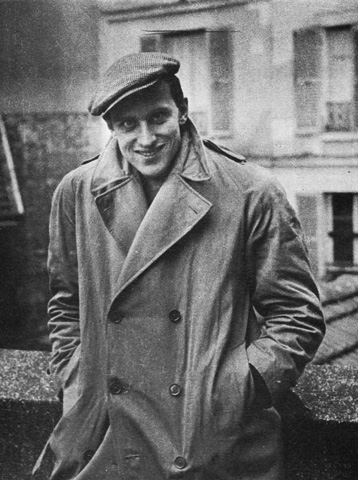
\includegraphics[height=3cm]{\PIXPATH/frontPage}
\end{center}

\vfill
\pagebreak

% Table of contents 
\tableofcontents
\vfill
\pagebreak

    % Fichier ./docs/tex/1.partie1.tex

% Partie 1: présentation du personnage

\section{Boris Vian, Bison Ravi, et tout leurs amis}

% Intro

Il est difficile de parler de Boris Vian. Peut-être parce qu'il
est difficile de lui coller une seule étiquette. Un seul nom,
même. «Boris Vian» pour l'état civil, «Bison Ravi» -- anagramme
de «Boris Vian» pour les proches, «Vernom Sullivan» pour certains
livres, et des dizaines d'autres pseudonymes en tant que chroniqueur.
% TODO: lien liste des pseudonymes (annexes ?)
Mais pour évoquer le personnage, on peut déjà s'intéresser à l'Histoire,
et à son histoire.
% TODO: Annexe frise chrono ?

\subsection{Contexte historique}


\subsection{Famille et éducation}


\subsection{Vie publique, vie privée}


% The end
\end{document}

